\section{Results and Analysis}
\subsection{Timing remarks and methodology}
All the following results were obtained on relatively old hardware: a NVIDIA Geforce GTX 1080ti with 11GB of GDDR5X memory, paired with an Intel Core i7-8700K CPU @ 4.8 GHz and 32GB of DDR4 RAM and the pc runs ubuntu 24.04.3 LTS. The point cloud used for testing contains 648433 points, representing a dense scan of an urban environment.
\subsection{General Observations}
The voxelizers are compared among five voxel sizes (0.25, 0.5, 0.75, 1.0, 1.25). For each voxel size, eight block sizes were tested (1, 2, 4, 8, 16, 32, 64, 256, 512, 1024 threads per block). The hash-table voxelizer was evaluated with three different capacity factors (2, 3, and 4 times the number of input points). The performance metrics recorded include total execution time and a breakdown of time spent in key phases of each algorithm.
Every configuration was run 100 times to obtain an average execution time, minimizing the impact of transient system load variations.

\subsection{Performance Analysis per Method}

\subsubsection{Morton-Code Voxelizer}
The Morton-based approach demonstrates consistent and predictable performance. Key findings include:

\begin{itemize}
    \item \textbf{Optimal block size:} 4--256 threads per block.
    \item \textbf{Total execution time:} Ranging from 25.18\,ms (voxel size 1.25, block size 64) to 40.46\,ms (voxel size 0.25, block size 1).
    \item \textbf{Primary bottleneck:} The sorting stage dominates runtime, requiring approximately 0.90--1.02\,ms, nearly constant across all tests.
\end{itemize}

Very small block sizes (1--4 threads) significantly slow down Morton-code generation (0.27--1.07\,ms), while larger block sizes stabilize this step to around 0.04\,ms.

\subsubsection{Hash-Table Voxelizer}
The hash-based method demonstrates greater variability, largely influenced by the selected capacity factor of the hash table.

\paragraph{Capacity Factor 2 (highest efficiency)}
\begin{itemize}
    \item \textbf{Best overall performance:} 25.67\,ms (voxel size 1.0, block size 32).
    \item \textbf{Optimal block sizes:} 8--32 threads per block.
    \item \textbf{Advantages:} Lowest memory overhead and fastest device-to-host transfer times.
\end{itemize}

\paragraph{Capacity Factor 3 (balanced)}
\begin{itemize}
    \item Execution times are \textbf{2--4\,ms slower} compared to capacity factor 2.
    \item Reduced collisions during accumulation, at the cost of increased memory usage.
\end{itemize}

\paragraph{Capacity Factor 4 (highest overhead)}
\begin{itemize}
    \item \textbf{5--10\,ms slower} than capacity factor 2.
    \item Initialization and memory operations increase disproportionately.
    \item Device-to-host + cleanup time rises up to 5.26\,ms (compared to 2.71\,ms for CF=2).
\end{itemize}

\subsection{Impact of Voxel Size}
Smaller voxel sizes generate a significantly larger number of unique voxel entries. This favors the hash-table method with a low capacity factor, as the Morton approach becomes less efficient when spatial data is highly fragmented.

For larger voxels (e.g., voxel size 1.25), the Morton method benefits from predictable spatial coherence and memory access patterns, making it more efficient than the hash-based approach.

\subsection{Impact of Block Size}
\begin{itemize}
    \item \textbf{Block sizes 1--4:} Strong performance penalties due to insufficient warp utilization.
    \item \textbf{Block sizes 8--256:} Optimal performance range with minimal overhead.
    \item \textbf{Block sizes 512--1024:} No significant improvements; potentially limited by register pressure.
\end{itemize}

\subsection{Timing Breakdown}

\subsubsection{Morton Method}
Dominant phases:
\begin{enumerate}
    \item \textbf{Sorting:} 0.90--1.02\,ms (consistent across tests)
    \item \textbf{Morton code computation:} 0.04--1.07\,ms (strongly dependent on block size)
    \item \textbf{Point accumulation:} 0.24--1.08\,ms
\end{enumerate}

\subsubsection{Hash Method}
Dominant phases:
\begin{enumerate}
    \item \textbf{Device-to-host transfer + cleanup:} 2.71--5.26\,ms (increases with capacity factor)
    \item \textbf{Initialization:} 0.33--3.71\,ms (proportional to hash-table size)
    \item \textbf{Populate phase:} 0.31--2.46\,ms (collision-sensitive)
\end{enumerate}

\subsection{Conclusions}

\subsubsection{Optimal Configurations}
The analysis indicates that different voxel sizes benefit from different GPU strategies:

\begin{itemize}
    \item \textbf{Small voxel sizes (0.25--0.5):} Hash-based voxelizer with capacity factor 2 and a block size of 16--32 threads.
    \item \textbf{Medium voxel sizes (0.75--1.0):} Hash-based voxelizer with capacity factor 2 and a block size of 32 threads.
    \item \textbf{Large voxel sizes (1.25 and above):} Morton-code voxelizer with a block size between 64 and 256 threads.
\end{itemize}

\subsubsection{Explanation}
These optimal configurations follow from the observed behaviour of both voxelization methods:

\begin{enumerate}
    \item For small voxel sizes, the hash method with capacity factor 2 achieves the highest throughput due to low memory overhead and efficient device-to-host transfers.
    \item For larger voxel sizes, the Morton-based approach becomes more efficient thanks to spatial coherence and predictable memory access patterns.
    \item Block sizes between 16 and 64 threads provide the most balanced performance in terms of occupancy and register usage.
\end{enumerate}

\subsubsection{Performance Limitations}
Despite their strengths, both methods exhibit certain limitations:

\begin{itemize}
    \item The hash-based method is primarily constrained by memory bandwidth, especially during device-to-host transfers.
    \item The Morton-based method is strongly dominated by the sorting stage, which forms its main computational bottleneck.
    \item For both approaches, increasing block sizes beyond 256 threads yields minimal benefits due to hardware saturation.
\end{itemize}

\subsection {gpu vs cpu performance}
% Comparison: CPU vs Minimum GPU Time (Morton and Hash methods)
\begin{table}[H]
\centering

\begin{tabular}{|c|c|c|c|c|c|}
\hline
\textbf{Voxel Size} & \textbf{CPU (ms)} & \textbf{Morton (ms)} & \textbf{Hash CF2 (ms)} & \textbf{Hash CF3 (ms)} & \textbf{Hash CF4 (ms)} \\
\hline
0.25 & 429.09 & 36.61 & 27.70 & 29.57 & 29.10 \\
0.5 & 335.89 & 29.14 & 26.20 & 28.30 & 28.57 \\
0.75 & 272.39 & 27.11 & 25.89 & 26.57 & 27.74 \\
1.0 & 253.67 & 25.71 & 25.67 & 26.99 & 27.46 \\
1.25 & 240.00 & 25.18 & 25.85 & 27.24 & 28.28 \\
\hline
\end{tabular}
\caption{CPU vs Minimum GPU Voxelization Time - All Methods}
\end{table}

% Comparison: CPU vs Maximum GPU Time (Morton and Hash methods)
\begin{table}[H]
\centering

\begin{tabular}{|c|c|c|c|c|c|}
\hline
\textbf{Voxel Size} & \textbf{CPU (ms)} & \textbf{Morton (ms)} & \textbf{Hash CF2 (ms)} & \textbf{Hash CF3 (ms)} & \textbf{Hash CF4 (ms)} \\
\hline
0.25 & 429.09 & 40.46 & 35.25 & 37.48 & 41.82 \\
0.5 & 335.89 & 31.18 & 33.87 & 35.53 & 40.00 \\
0.75 & 272.39 & 28.62 & 33.80 & 36.09 & 39.12 \\
1.0 & 253.67 & 27.63 & 33.36 & 35.26 & 38.53 \\
1.25 & 240.00 & 28.64 & 34.41 & 36.85 & 39.06 \\
\hline
\end{tabular}
\caption{CPU vs Maximum GPU Voxelization Time - All Methods}
\end{table}

The above tables demonstrate substantial performance improvements when using GPU-based voxelization compared to CPU implementations. Across all tested voxel sizes, the best-performing GPU configurations achieve speedup factors ranging from 9.5× to 15.5×, with the most significant gains observed at smaller voxel sizes where parallelization is most effective. Even in the worst-case GPU scenarios (maximum execution times), the speedup remains impressive at 6.1× to 12.2× faster than CPU execution. The hash-based method with capacity factor 2 consistently delivers optimal performance, achieving minimum execution times between 25.67ms and 27.70ms compared to CPU times of 240.00ms to 429.09ms. Notably, the speedup factor decreases slightly as voxel size increases, suggesting that GPU implementations particularly excel when processing larger numbers of smaller voxels, where the massive parallelism of the GPU architecture can be fully exploited.
\subsection{Figures of the overall gpu times}
% Requires pgfplots package
% Add to preamble: \usepackage{pgfplots}
% \pgfplotsset{compat=1.17}

% GRAPH 1: Voxel Size 0.25
\begin{figure}[H]
\centering
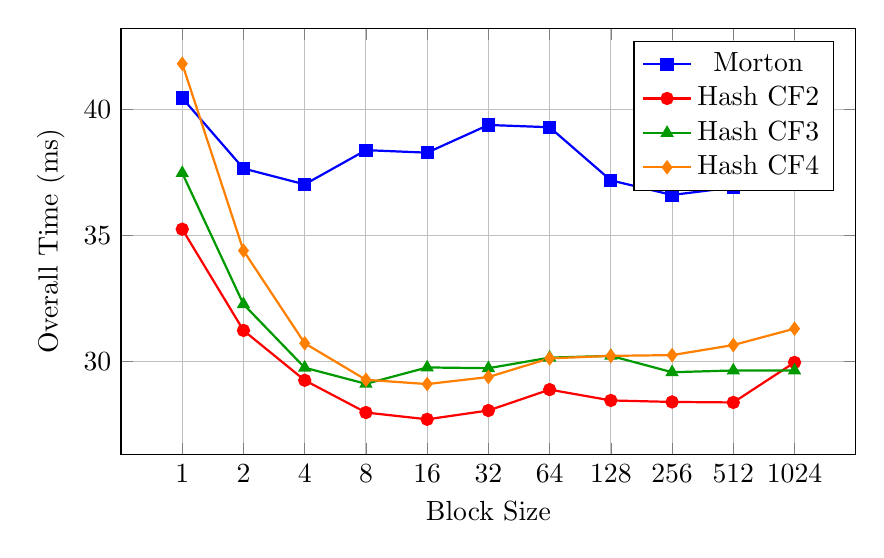
\begin{tikzpicture}
\begin{axis}[
    width=0.9\textwidth,
    height=7cm,
    xlabel={Block Size},
    ylabel={Overall Time (ms)},
    legend pos=north east,
    xmode=log,
    log basis x={2},
    xtick={1,2,4,8,16,32,64,128,256,512,1024},
    xticklabels={1,2,4,8,16,32,64,128,256,512,1024},
    grid=major,
    mark size=2pt,
]

% Morton
\addplot[color=blue,mark=square*,thick] coordinates {
    (1,40.46) (2,37.66) (4,37.03) (8,38.39) (16,38.29) 
    (32,39.39) (64,39.30) (128,37.19) (256,36.61) (512,36.91) (1024,39.67)
};

% Hash CF2
\addplot[color=red,mark=*,thick] coordinates {
    (1,35.25) (2,31.23) (4,29.25) (8,27.97) (16,27.70) 
    (32,28.05) (64,28.88) (128,28.45) (256,28.39) (512,28.37) (1024,29.96)
};

% Hash CF3
\addplot[color=green!60!black,mark=triangle*,thick] coordinates {
    (1,37.48) (2,32.27) (4,29.75) (8,29.11) (16,29.76) 
    (32,29.73) (64,30.15) (128,30.22) (256,29.57) (512,29.64) (1024,29.64)
};

% Hash CF4
\addplot[color=orange,mark=diamond*,thick] coordinates {
    (1,41.82) (2,34.40) (4,30.72) (8,29.27) (16,29.10) 
    (32,29.38) (64,30.12) (128,30.22) (256,30.25) (512,30.65) (1024,31.30)
};

\legend{Morton, Hash CF2, Hash CF3, Hash CF4}
\end{axis}
\end{tikzpicture}
\caption{Overall execution time for voxel size 0.25}
\end{figure}

% GRAPH 2: Voxel Size 0.5
\begin{figure}[H]
\centering
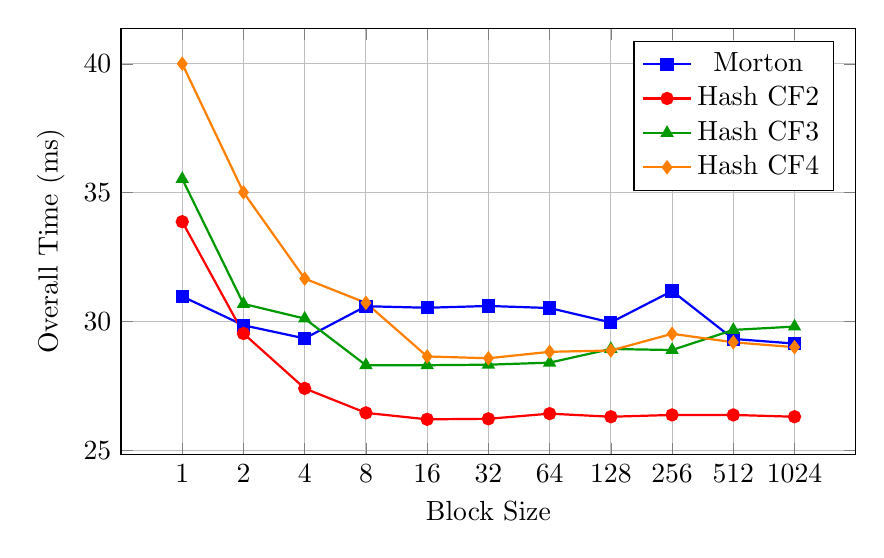
\begin{tikzpicture}
\begin{axis}[
    width=0.9\textwidth,
    height=7cm,
    xlabel={Block Size},
    ylabel={Overall Time (ms)},
    legend pos=north east,
    xmode=log,
    log basis x={2},
    xtick={1,2,4,8,16,32,64,128,256,512,1024},
    xticklabels={1,2,4,8,16,32,64,128,256,512,1024},
    grid=major,
    mark size=2pt,
]

% Morton
\addplot[color=blue,mark=square*,thick] coordinates {
    (1,30.97) (2,29.85) (4,29.34) (8,30.59) (16,30.53) 
    (32,30.60) (64,30.52) (128,29.96) (256,31.18) (512,29.32) (1024,29.14)
};

% Hash CF2
\addplot[color=red,mark=*,thick] coordinates {
    (1,33.87) (2,29.53) (4,27.40) (8,26.45) (16,26.20) 
    (32,26.22) (64,26.42) (128,26.30) (256,26.37) (512,26.37) (1024,26.30)
};

% Hash CF3
\addplot[color=green!60!black,mark=triangle*,thick] coordinates {
    (1,35.53) (2,30.68) (4,30.11) (8,28.30) (16,28.30) 
    (32,28.32) (64,28.40) (128,28.93) (256,28.89) (512,29.67) (1024,29.80)
};

% Hash CF4
\addplot[color=orange,mark=diamond*,thick] coordinates {
    (1,40.00) (2,35.01) (4,31.66) (8,30.72) (16,28.64) 
    (32,28.57) (64,28.82) (128,28.87) (256,29.52) (512,29.19) (1024,29.00)
};

\legend{Morton, Hash CF2, Hash CF3, Hash CF4}
\end{axis}
\end{tikzpicture}
\caption{Overall execution time for voxel size 0.5}
\end{figure}

% GRAPH 3: Voxel Size 0.75
\begin{figure}[H]
\centering
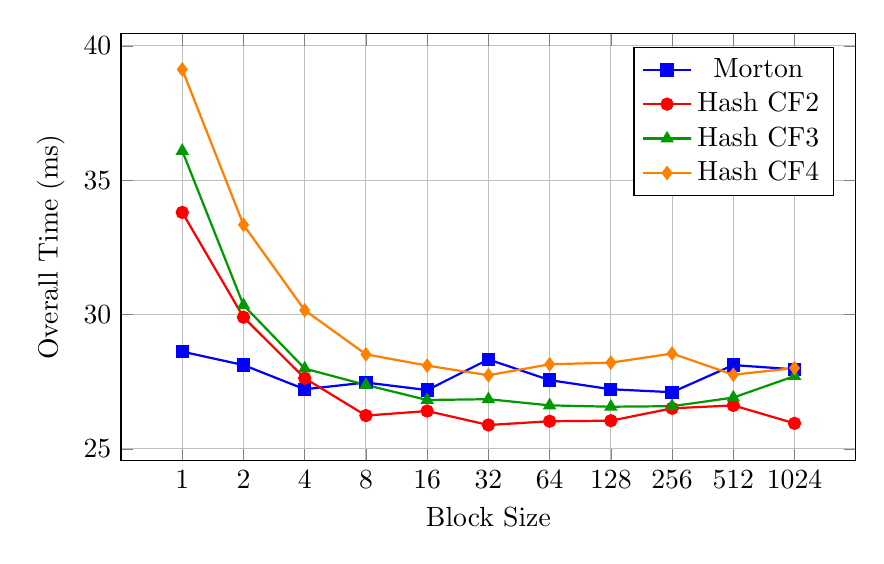
\begin{tikzpicture}
\begin{axis}[
    width=0.9\textwidth,
    height=7cm,
    xlabel={Block Size},
    ylabel={Overall Time (ms)},
    legend pos=north east,
    xmode=log,
    log basis x={2},
    xtick={1,2,4,8,16,32,64,128,256,512,1024},
    xticklabels={1,2,4,8,16,32,64,128,256,512,1024},
    grid=major,
    mark size=2pt,
]

% Morton
\addplot[color=blue,mark=square*,thick] coordinates {
    (1,28.62) (2,28.12) (4,27.22) (8,27.47) (16,27.19) 
    (32,28.33) (64,27.56) (128,27.22) (256,27.11) (512,28.12) (1024,27.96)
};

% Hash CF2
\addplot[color=red,mark=*,thick] coordinates {
    (1,33.80) (2,29.90) (4,27.63) (8,26.24) (16,26.41) 
    (32,25.89) (64,26.03) (128,26.05) (256,26.51) (512,26.62) (1024,25.95)
};

% Hash CF3
\addplot[color=green!60!black,mark=triangle*,thick] coordinates {
    (1,36.09) (2,30.35) (4,27.99) (8,27.38) (16,26.82) 
    (32,26.85) (64,26.62) (128,26.57) (256,26.59) (512,26.91) (1024,27.71)
};

% Hash CF4
\addplot[color=orange,mark=diamond*,thick] coordinates {
    (1,39.12) (2,33.34) (4,30.16) (8,28.52) (16,28.10) 
    (32,27.74) (64,28.15) (128,28.21) (256,28.55) (512,27.76) (1024,28.01)
};

\legend{Morton, Hash CF2, Hash CF3, Hash CF4}
\end{axis}
\end{tikzpicture}
\caption{Overall execution time for voxel size 0.75}
\end{figure}

% GRAPH 4: Voxel Size 1.0
\begin{figure}[H]
\centering
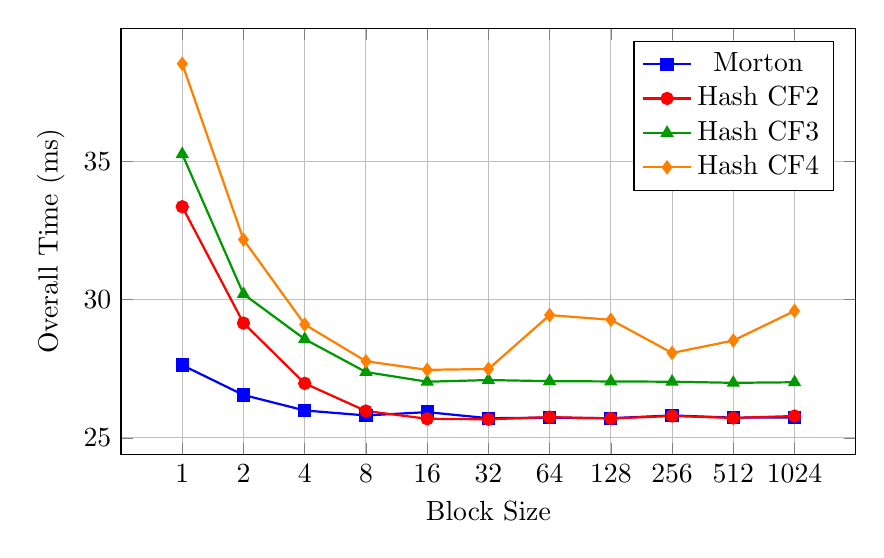
\begin{tikzpicture}
\begin{axis}[
    width=0.9\textwidth,
    height=7cm,
    xlabel={Block Size},
    ylabel={Overall Time (ms)},
    legend pos=north east,
    xmode=log,
    log basis x={2},
    xtick={1,2,4,8,16,32,64,128,256,512,1024},
    xticklabels={1,2,4,8,16,32,64,128,256,512,1024},
    grid=major,
    mark size=2pt,
]

% Morton
\addplot[color=blue,mark=square*,thick] coordinates {
    (1,27.63) (2,26.55) (4,25.99) (8,25.81) (16,25.93) 
    (32,25.71) (64,25.73) (128,25.71) (256,25.81) (512,25.73) (1024,25.74)
};

% Hash CF2
\addplot[color=red,mark=*,thick] coordinates {
    (1,33.36) (2,29.15) (4,26.97) (8,25.97) (16,25.69) 
    (32,25.67) (64,25.75) (128,25.70) (256,25.79) (512,25.72) (1024,25.79)
};

% Hash CF3
\addplot[color=green!60!black,mark=triangle*,thick] coordinates {
    (1,35.26) (2,30.20) (4,28.57) (8,27.38) (16,27.03) 
    (32,27.09) (64,27.05) (128,27.04) (256,27.03) (512,26.99) (1024,27.01)
};

% Hash CF4
\addplot[color=orange,mark=diamond*,thick] coordinates {
    (1,38.53) (2,32.17) (4,29.10) (8,27.77) (16,27.46) 
    (32,27.49) (64,29.44) (128,29.27) (256,28.07) (512,28.52) (1024,29.59)
};

\legend{Morton, Hash CF2, Hash CF3, Hash CF4}
\end{axis}
\end{tikzpicture}
\caption{Overall execution time for voxel size 1.0}
\end{figure}

% GRAPH 5: Voxel Size 1.25
\begin{figure}[H]
\centering
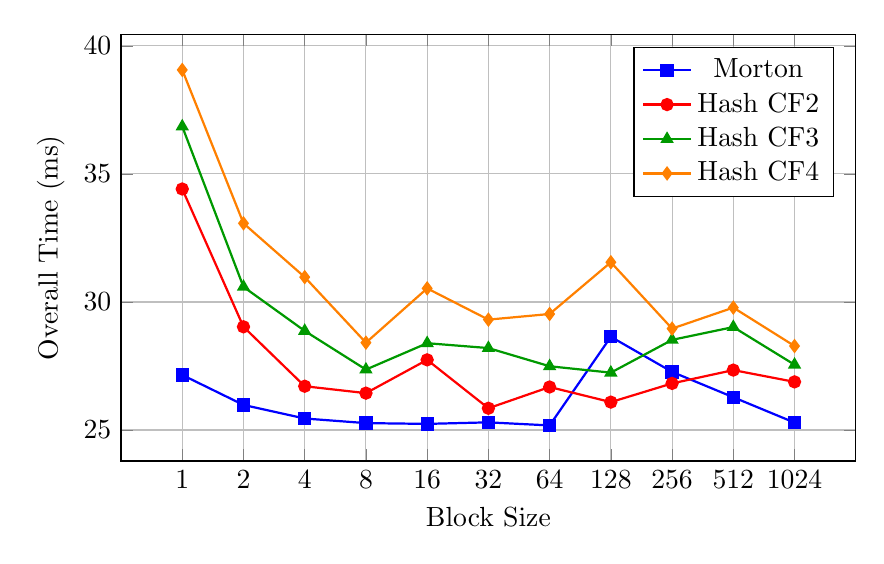
\begin{tikzpicture}
\begin{axis}[
    width=0.9\textwidth,
    height=7cm,
    xlabel={Block Size},
    ylabel={Overall Time (ms)},
    legend pos=north east,
    xmode=log,
    log basis x={2},
    xtick={1,2,4,8,16,32,64,128,256,512,1024},
    xticklabels={1,2,4,8,16,32,64,128,256,512,1024},
    grid=major,
    mark size=2pt,
]

% Morton
\addplot[color=blue,mark=square*,thick] coordinates {
    (1,27.15) (2,25.98) (4,25.45) (8,25.27) (16,25.24) 
    (32,25.30) (64,25.18) (128,28.64) (256,27.27) (512,26.28) (1024,25.29)
};

% Hash CF2
\addplot[color=red,mark=*,thick] coordinates {
    (1,34.41) (2,29.03) (4,26.71) (8,26.44) (16,27.74) 
    (32,25.85) (64,26.68) (128,26.09) (256,26.82) (512,27.34) (1024,26.88)
};

% Hash CF3
\addplot[color=green!60!black,mark=triangle*,thick] coordinates {
    (1,36.85) (2,30.59) (4,28.87) (8,27.36) (16,28.39) 
    (32,28.20) (64,27.49) (128,27.24) (256,28.52) (512,29.02) (1024,27.55)
};

% Hash CF4
\addplot[color=orange,mark=diamond*,thick] coordinates {
    (1,39.06) (2,33.07) (4,30.97) (8,28.41) (16,30.53) 
    (32,29.31) (64,29.53) (128,31.55) (256,28.96) (512,29.78) (1024,28.28)
};

\legend{Morton, Hash CF2, Hash CF3, Hash CF4}
\end{axis}
\end{tikzpicture}
\caption{Overall execution time for voxel size 1.25}
\end{figure}